

\documentclass[12pt]{report}
\usepackage[utf8]{inputenc}
\usepackage[russian]{babel}
\usepackage[14pt]{extsizes}
\usepackage{listings}
\usepackage{graphicx}
\usepackage{amsmath,amsfonts,amssymb,amsthm,mathtools} 
\usepackage{pgfplots}
\usepackage{filecontents}
\usepackage{float}
\usepackage{indentfirst}
\usepackage{eucal}
\usepackage{enumitem}
%s\documentclass[openany]{book}
\frenchspacing

\usepackage{titlesec}
\titleformat{\section}
{\normalsize\bfseries}
{\thesection}
{1em}{}
\titlespacing*{\chapter}{0pt}{-30pt}{8pt}
\titlespacing*{\section}{\parindent}{*4}{*4}
\titlespacing*{\subsection}{\parindent}{*4}{*4}

\usepackage{indentfirst} % Красная строка

\usetikzlibrary{datavisualization}
\usetikzlibrary{datavisualization.formats.functions}

\usepackage{amsmath}

\usepackage{amssymb}

% Для листинга кода:
\lstset{ %
	language=lisp,                 % выбор языка для подсветки (здесь это С)
	texcl=true,
	extendedchars=\true,
	basicstyle=\small\sffamily, % размер и начертание шрифта для подсветки кода
	numbers=left,               % где поставить нумерацию строк (слева\справа)
	numberstyle=\tiny,           % размер шрифта для номеров строк
	stepnumber=1,                   % размер шага между двумя номерами строк
	numbersep=5pt,                % как далеко отстоят номера строк от подсвечиваемого кода
	showspaces=false,            % показывать или нет пробелы специальными отступами
	showstringspaces=false,      % показывать или нет пробелы в строках
	showtabs=false,             % показывать или нет табуляцию в строках
	frame=single,              % рисовать рамку вокруг кода
	tabsize=2,                 % размер табуляции по умолчанию равен 2 пробелам
	captionpos=t,              % позиция заголовка вверху [t] или внизу [b] 
	breaklines=true,           % автоматически переносить строки (да\нет)
	breakatwhitespace=false, % переносить строки только если есть пробел
	escapeinside={\#*}{*)},  % если нужно добавить комментарии в коде
	%inputencoding=utf8x,
	%extendedchars=\true
}



\usepackage[left=2cm,right=2cm, top=2cm,bottom=2cm,bindingoffset=0cm]{geometry}
% Для измененных титулов глав:
\usepackage{titlesec, blindtext, color} % подключаем нужные пакеты
\definecolor{gray75}{gray}{0.75} % определяем цвет
\newcommand{\hsp}{\hspace{20pt}} % длина линии в 20pt
% titleformat определяет стиль
\titleformat{\chapter}[hang]{\Huge\bfseries}{\thechapter\hsp\textcolor{gray75}{|}\hsp}{0pt}{\Huge\bfseries}


% plot
\usepackage{pgfplots}
\usepackage{filecontents}
\usepackage[unicode, pdftex]{hyperref}
\usetikzlibrary{datavisualization}
\usetikzlibrary{datavisualization.formats.functions}

 
\begin{document}



\url{https://github.com/Winterpuma/bmstu_FaLP/tree/master/CommonLisp/theory}

\url{https://github.com/Winterpuma/bmstu_FaLP/wiki}

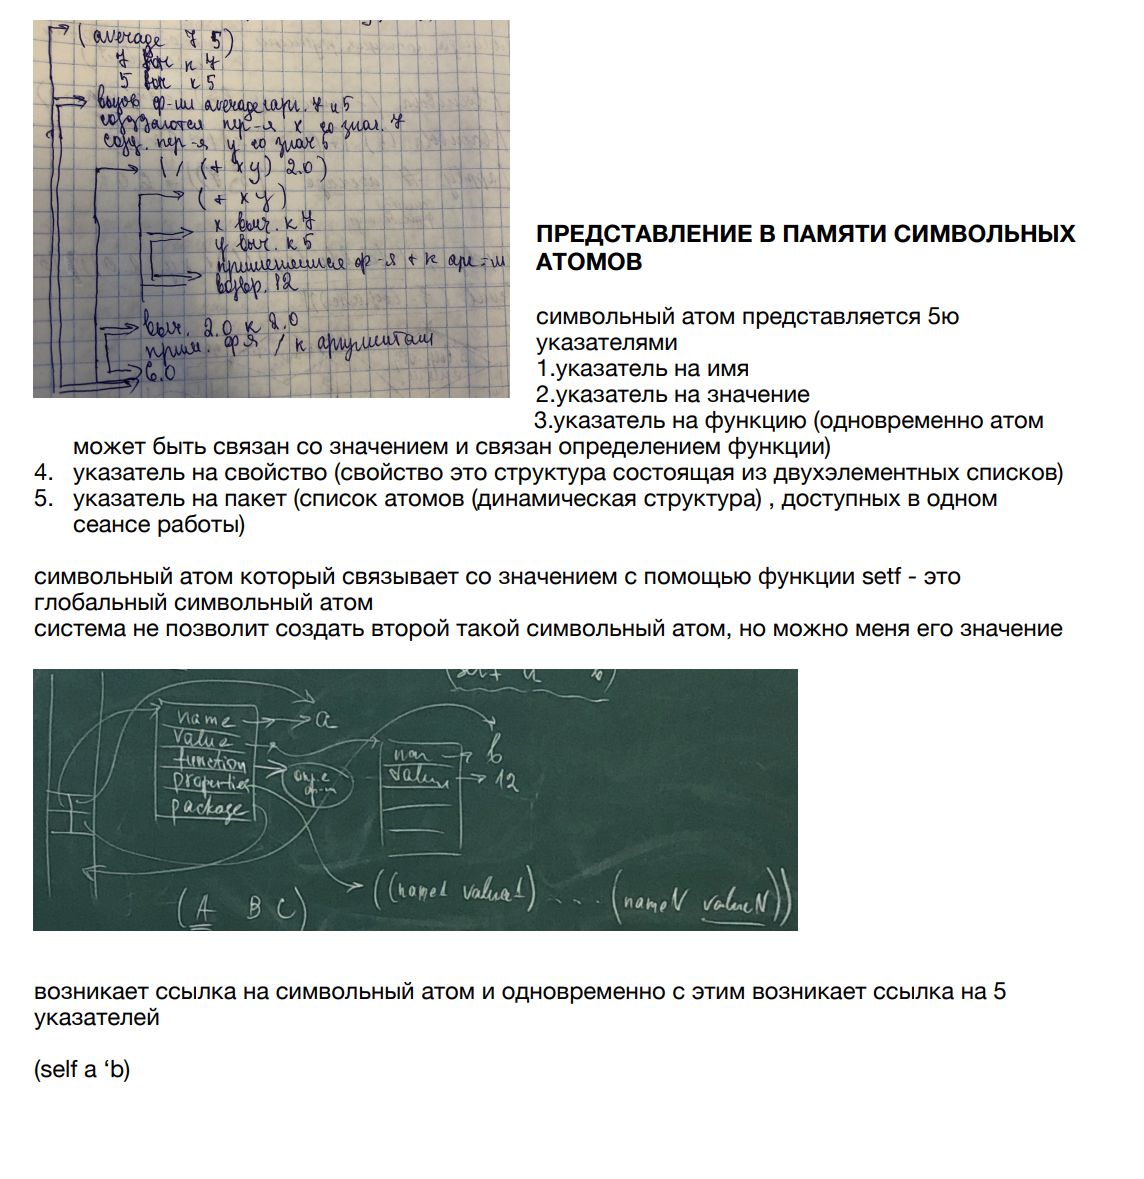
\includegraphics[scale=1]{img/1}

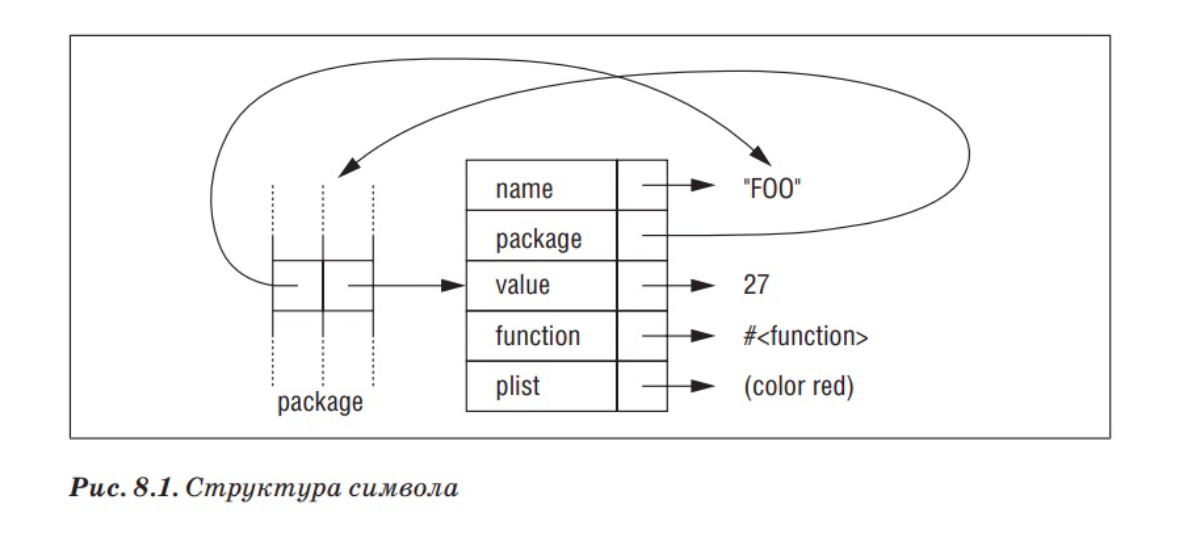
\includegraphics[scale=1]{img/2}

\section*{Базис Lisp}
	
Базис -- это минимальный набор инструментов языка и стркутур данных, который позволяет решить любые задачи.


Базис Lisp :

\begin{itemize}
	\item атомы (представляются в памяти пятью указателями  --  name, value, function, property, package) и структуры (представляющиеся бинарными узлами);
	\item базовые (несколько) функций, функционалов и форм: встроенные — примитивные функции (atom, eq, cons, car, cdr); формы (quote, cond, lambda, eval); функционалы (apply, funcall).
\end{itemize}

Атомы:
\begin{itemize} 
	\item символы (идентификаторы) – синтаксически – набор литер (букв и цифр), начинающихся с буквы;
	\item специальные символы – {T, Nil} (используются для обозначения логических констант);
	\item самоопределимые атомы – натуральные числа, дробные числа, вещественные числа, строки – последовательность символов, заключенных в двойные апострофы (например, “abc”);
\end{itemize} 

Более сложные данные – списки и точечные пары (структуры), которые строятся с помощью унифицированных структур – блоков памяти – бинарных узлов.

Определения:

Точечная пара ::= (<атом> . <атом>) | (<атом> . <точечная пара>) | (<точечная пара> . <атом>) | (<точечная пара> . <точечная пара>);

Список ::= <пустой список> | <непустой список>, где 

<пустой список> ::= () | Nil,

<непустой список> ::= (<первый элемент> . <хвост>),

<первый элемент> ::= <S-выражение>,

S-выражение ::= <атом> | <точечная пара>,

<хвост> ::= <список>.


Функцией называется правило, по которому каждому значению одного или нескольких  аргументов ставится в соответствие конкретное значение результата. 

%Функции всюду определены (то есть результат есть всегда), их аргументы и результаты -- S-выражения.

Функционалом, или функцией высшего порядка называется функция, аргументом или  результатом которой является другая функция.

Форма -- функция, которая особым образом обрабатывает свои аргументы, т. е. требует специальной обработки. Переменное число аргументов или они обрабатывются/не обрабатываются по-разному.

%Форма, или вычислимое выражение – это атом или список, который можно  вычислить и получить значение.


Синтаксически:

любая структура (точечная пара или список) заключается в круглые скобки: (A . B) – точечная пара, (A) – список из одного элемента. Пустой список изображается как Nil или ();

непустой список по определению может быть изображен: (A . (B . (C . (D . ())))),  допустимо изображение списка последовательностью атомов, разделенных пробелами – (A B C D).

Элементы списка могут быть списками (любой список заключается в круглые скобки), например – (A (B C) (D С)). Таким образом, синтаксически наличие скобок является признаком структуры – списка или точечной пары.

Любая непустая структура Lisp в памяти представляется списковой ячейкой, хранящей два указателя: на голову (первый элемент) и хвост – всё остальное. Точечная пара в памяти представляется бинарным узлом.



Отличительные особенности Lisp: только символьная обработка; все можно представить в виде функций.
	
Вся информация (данные и программы) в Lisp представляется в виде символьных выражений – S-выражений. 

По определению: S-выражение ::= <атом> | <точечная пара>.
	
В зависимости от контекста одни и те же объекты могут играть роль переменных или констант, причем значения и того, и другого могут быть произвольной сложности. Если объект играет роль константы, то для объявления константы достаточно заблокировать его вычисление, то есть как бы взять его в кавычки, отмечающие буквально используемые фразы, не требующие обработки. 

Апостроф – сокращённое обозначение функции quote.

quote - блокирует вычисление своего аргумента. В качестве своего значения выдаёт сам аргумент, не вычисляя его. Перед константами - числами и атомами T, Nil можно не ставить апостроф.

\section*{Синтаксическая форма и хранение программы в памяти}

Программа на Lisp представляет собой вызов функции на верхнем уровне. Все операции над данными оформляются и  записываются как функции, которые имеют значение, даже если их основное предназначение – осуществление некоторого побочного эффекта. Программа является ничем иным, как набором запрограммированных функций.

\textbf{Синтаксически} программа оформляется в виде S-выражения (обычно -- списка -- частного случая точечной пары), которое очень часто может быть структурированным. Наличие скобок является признаком структуры. 



Атомы представляются \textbf{в памяти} пятью указателями  (name, value, function, property, package), а любая непустая структура --  списковой ячейкой (бинарным узлом), хранящей два указателя: на голову (первый элемент) и хвост -- все остальное.


\section*{Трактовка элементов списка.}

По определению списка, приведенному выше: если список непустой, то он представляет из себя точечную пару из  <первого элемента> и <хвоста>, где <первый элемент> -- это <S-выражение>, а <хвост> -- это <список>.

Список можно вычислить, если он представляет собой обращение к  функции, или функциональный вызов: (f e1 e2 … en), где f – символьный атом, имя вызываемой функции; e1, e2, …, en – аргументы этой функции; n - число аргументов функции.

В случае n=0 имеем вызов функции без аргументов: (f). Обычно e1, e2, …, en являются вычислимыми выражениями и вычисляются последовательно слева направо.

Таким образом, если в процессе работы лисп-интерпретатора  требуется вычислить некоторый список, то первым элементом этого   списка должно быть имя функции. Если это не так, лисп-интерпретатор  сообщает об ошибке и прерывает вычисление текущего выражения  программы.


\section*{Порядок реализации программы.}

Типичная лисп-программа включает:
\begin{itemize}
	\item определения новых функций на базе встроенных функций и других функций, определённых в этой программе;
	\item {вызовы этих новых функций для конкретных значений их аргументов.}
\end{itemize}

Как отмечалось выше, программа на Lisp представляет собой вызов функции на верхнем уровне и синтаксически оформляется в виде S-выражения. Вычисление программы реализует лисп-интерпретатор, который считывает очередную входящую в программу форму, вычисляет её (анализирует функцией eval) и выводит полученный результат (S-выражение).

Eval выполняет двойное  вычисление своего аргумента. Эта функция является обычной, и первое  вычисление аргумента выполняет так же, как и любая обычная функция.  Полученное при этом выражение вычисляется ещё раз. Такое двойное  вычисление может понадобиться либо для снятия блокировки вычислений (установленной функцией quote), либо же для вычисления сформированного в ходе первого вычисления нового функционального вызова.


Вызов (eval S-выражение):

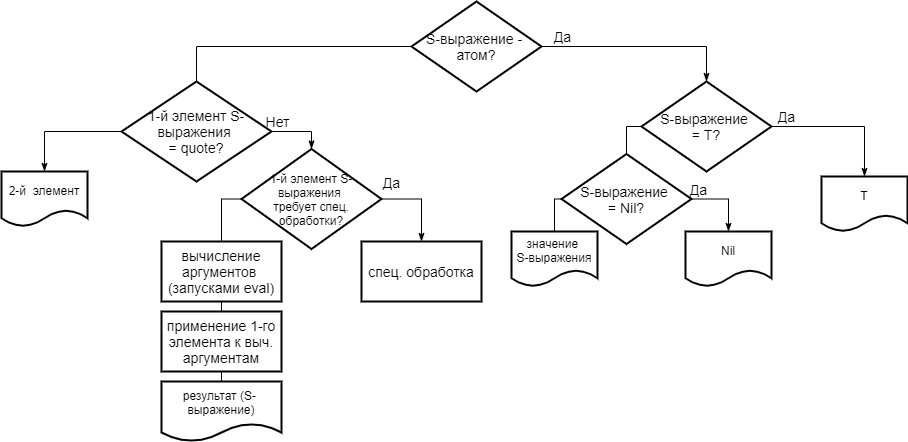
\includegraphics[scale=0.5]{img/eval}

\section*{Классификация функций}


Функции -- лишь логическая интерпретация, а синтаксически все одинаково.

Функции делятся на базисные или небазисные, и по способу реализации (чистые математические и тд)

Формальные параметры -- символьные атомы. Когда задаем фактиеские параметры, должна быть выделена память. Лексическая переменная -- символьный атом. Распределение памяти автоматиччески в нужный момент.



\begin{enumerate}
	\item Чистые  математические функции (имеют фиксированное количество аргументов, сначала выяисляются все аргументы, а только потом к ним применяется функция);
	\item Рекурсивные функции (основной способ выполнения повторных вычислений);
	\item Специальные функции, или формы (могут принимать произвольное количество аргументов, или аргументы могут обрабатываться по-разному);
	\item Псевдофункции (создают «эффект», например, вывод на экран);
	\item Функции с вариантами значений, из которых выбирается одно;
	\item Функции высших порядков, или функционалы --  функции, аргументом или  результатом которых является другая функция (используются для построения синтаксически управляемых программ);
\end{enumerate}

Классификаци базисных функций и функций ядра.

\begin{enumerate}
	\item Селекторы: car и cdr (будут подробнее расссмотрены ниже).
	\item Конструкторы: cons и list (будут подробнее расссмотрены ниже).
	\item Предикаты -- <<логические>> функции, позволяющие определить структуру элемента:
	\begin{itemize}
		\item atom возвращает T, если значением её единственного аргумента является атом, иначе -- NIL;
		\item null возвращает T, если значение его аргумента -- NIL (пустой список), иначе -- NIL;
		\item listp возвращает T, если значением её аргумента является список, иначе -- NIL;
		\item consp возвращает T, если значением её аргумента является структура, представленная в виде списковой ячейки, иначе -- NIL. 
	\end{itemize}
	\item Функции сравнения (принимают два аргумента, перечислены по мере роста <<тщательности>> проверки):
	\begin{itemize}
		\item eq корректно сравнивает два символьных атома. Так как атомы не дублирутюся для данного сеанса работы, то фактически сравниваются соответсвующие указатели. 
		Возвращает T, когда: 1) значением одного из аргументов является атом, и одновременно 2) значения аргументов равны (идентичны). В ином случае значением функции eq является NIL. (eq  'ab 'Ab) => T, но (eq 1 2) => NIL.
		\item eql корректно сравнивает атомы и числа одинакового типа (синтетической формы записи). Например, (eql 1 1) вернет T, а (eql 1 1.0) -- Nil, так как целое значение 1 и значение с плавающей точкой 1.0 являются представителями различных классов;
		\item = корректно сравнивает только числа, причем числа могут быть разных типов. Например, и (= 1 1), и (= 1 1.0) вернет T;
		\item equal работает идентично eql, но в дополнение умеет корректно сравнивать списки (считая списки эквивалентными, если они рекурсивно, согласно тому же equal, имеют одинаковую структуру и содержимое; считая строки эквивалентными, если они содержат одинаковые знаки);
		\item equalp корректно сравнивает любые S-выражения. 
	\end{itemize}
\end{enumerate}
	

\section*{Функционалы}
 В Lisp используются применяющие и отображающие функционалы, функционалы, являющиеся предикатами, функционалы, использующие предикаты в качестве функционального объекта.

Функционалы: 2 группы - Применяющие (apply,  funcall) и отображающие (mapcar, maplist)

Функция – всегда первый аргумент функционала



Применяющие: (apply \#'fun lst)--  fun-имя или lambda-выражение, lst -- список (фиксированное число), (funcall \#'fun arg1, ... argn) -- количество аргументов определяется fun.

Фиксирует окружение функции в момент, когда функция начала работать (может, в теле есть глобальные атомы)


Отображающие -  функционалы, которые позволяют реализовывать многократные или повторные вычисление (циклы).

(mapcar \#'fun lst) -- fun -- имя или lambda-выражение, к каждому элементу списка по верхнему уровню, на выходе -- список из результатов. функция должна уметь обрабатывать как атомы, так и списки получается

(maplist \#'fun lst) -- целиком к списку, к хвосту, к хвосту хвоста ..., функция должна работать со списками

Функция должна быть одноаргументной.

В результирующий список все объединяется функцией list. 

Fun должна быть одноаргументной. В предыдущих примерах. Чтобы использовать многоаргументные:

(mapcar \#’fun lst1 lst2 .. lstk)
Выбирает из каждого списка car-элементы и применяет функцию, затем – вторые (головы от хвостов). Проход по верхнему уровню. Закончится, когда закончатся элементы самого короткого списка. 

Аналогично maplist

Существуют аналоги maplist -- mapcon (mapcan -- mapcar), использующие структуроразрущающий nconc вместо list. Работает быстрее, НО результаты применения функций должны быть списками, для nconc.


\textbf{Find-if}

(функция или предикат)

(find-if  \#’predicat lst) - проходит по верхнему уровню списка и возвращает первый элемент, удовлетворяющий данному предикату

(find-if \#’odd. ‘(2 4 7 5)) -> 7

(find-if-not \#’predicat lst) – не удовлетворяющий

(find elem seq) -- просто ищет первый

\textbf{Remove-if}

(remove-if \#’predicat lst)
(remove-if-not \#’predicat lst)
(remove elem seq)

(возвращает список без всех элементов, которые (не) удовлетворяют условию)

\textbf{Reduce}

(reduce \#’fun lst)
Fun – как минимум 2-аргументная. Применяет функцию каскадным образом к элементам lst – 1 и 2, к результату и 3.


она выполняет отображение для одной последовательности, применяя функцию двух аргументов сначала к первым двум элементам последовательности, а после первого вызова, последовательно применяя ее к полученному результату и следующим элементам. Таким образом, следующее выражение сложит числа от единицы до десяти: (reduce \#'+ \#(1 2 3 4 5 6 7 8 9 10)) ==> 55

REDUCE является очень полезной функцией – когда вам нужно создать из последовательности одно значение, есть вероятность, что вы сможете сделать это с помощью REDUCE, и она часто приводит к лаконичной записи того, что вы хотите сделать. Например, для нахождения максимального значения в последовательности вы можете просто написать (reduce \#'max numbers). 


\textbf{every}

(every \#’predicat lst) – T если все элементы удовлетворяют предикату

\textbf{some}

(some \#’predicat lst) – T если некоторые

Другими полезными функциями являются EVERY, SOME, NOTANY и NOTEVERY, которые пробегают по элементам последовательности выполняя заданный предикат. Первым аргументом всех этих функций является предикат, а остальные аргументы – последовательности. Предикат должен получать столько аргументов, сколько последовательностей будет передано функциям. Элементы последовательностей передаются предикату (по одному элементу за раз) пока не закончатся элементы, или не будет выполнено условие завершения: 

EVERY завершается, возвращая ложное значение, сразу как это значение будет возвращено предикатом. Если предикат всегда возвращает истинное значение, то функция также вернет истинное значение.

SOME возвращает первое не NIL значение, возвращенное предикатом, или возвращает ложное значение, если предикат никогда не вернул истинного значения. 

NOTANY возвращает ложное значение, если предикат возвращает истинное значение, или истинное, если этого не произошло.

А NOTEVERY возвращает истинное значение сразу, как только предикат возвращает ложное значение, или ложное, если предикат всегда возвращал истинное. Вот примеры проверок для одной последовательности:

(every \#'evenp \#(1 2 3 4 5)) ==> NIL
(some \#'evenp \#(1 2 3 4 5)) ==> T
(notany \#'evenp \#(1 2 3 4 5)) ==> NIL
(notevery \#'evenp \#(1 2 3 4 5)) ==> T



\textbf{Примеры на использование функционалов}

Множество из списка

(defun consists-of (lst) (if (member (car lst) (cdr lst)) 1 0))

(defun all-last-element (lst)
(if (eql (consists-of lst). 0) (list (car lst)) ())))

(defun collection-to-set (lst)
(mapcon \#’all-last-element lst))

(collection-to-set ‘(I t I g t k s I f k)) -> (g t s I f k) – множество, но порядок «неожиданный»


Декартово произведение

(defun decart (listx listy) 
(mapcan \#’(lambda (x)
(mapcar \#’(lambda (y)
(list x y)) lsty))
Lstx))

\#’ нужно использовать во вложенной функции, чтобы зафиксировать значение x. На более высоком уровне. В ЛАБАХ ВСЕГДА ПИСАТЬ

При использовании функционального объекта должно быть использовано замыкание контекста функции, которым обеспечивается связывание свободных переменных со значениями.

(decart ‘(a b) ‘(1 2)). -> ((a 1) (a 2) (b 1) (b 2))



\section*{Структуроразрушающие и не разрушающие структуру списка функции}

Функции, работающие со списками, делятся на:
\begin{itemize}
	\item функции, не разрушающие структуру списка (сохраняется возможность работать с исходным списком);
	\item функции, разрушающие структуру списка (не сохраняется возможность работы с исходным списком, зато функция выполнятся быстрее по сравнению со своим не разрушающим аналогом, так как не создаются копии cons-ячеек).
\end{itemize}

Из-за такого разделения существует много дублирующих функций: функциям, не разрушающим структуру списка (reverse, substitute, ...) соответствуют структуроразрушающие функции, которые, как правило, начинаются с буквы <<n>>, как признак того, что не создаются копии (nreverse, nsubstitute, ...). conc является структуроразрушающим аналогом append, delete -- структуроразрушающим аналогом remove.

\section*{Способы создания функций}

Определение функций пользователя в Lisp-е возможно двумя способами.


\begin{itemize}
	\item Базисный способ  определения  функции - использование $\lambda$-выражения ($\lambda$-нотации). Так создаются функции без имени.
	
	$\lambda$-выражение: (lambda $\lambda$-список форма), 
	где $\lambda$-список --  это формальные параметры функции (список аргументов), а форма -- это тело функции.
	
	Вызов такой функции осуществляется следующим способом: ($\lambda$-выражение последовательность\_форм), 
	где последовательность\_форм -- это фактические параметры.
	
	Вычисление функций без имени может быть также выполнено с использованием функционала apply: (apply $\lambda$-выражение последовательность\_форм), где последовательность\_форм -- это список фактических параметров; или с использованием функционала funcall: (funcall $\lambda$-выражение последовательность\_форм), где последовательность\_форм -- это фактические параметры.
	
	Функционал apply является обычной функцией с двумя  вычисляемыми аргументами, обращение к ней имеет вид: (apply F L), где F – функциональный аргумент и L -- список, рассматриваемый как список фактических параметров для F. Значение функционала -- результат применения F к этим фактическим параметрам.
	
	Функционал funcall – особая функция с вычисляемыми аргументами, обращение к ней: (funcall F e1 … en), n $>= 0$. Её   действие аналогично apply, отличие состоит в том, что аргументы  применяемой функции F задаются не списком, а по отдельности. 
	
	funcall используется тогда, когда во время написания кода количество аргументов известно, apply -- когда неизвестно.
	
	\item Другой способ определения функции -- использование макро-определения defun: 
	
	(defun имя\_функции $\lambda$-выражение), 
	
	или  в облегченной форме:
	
	(defun имя\_функции $(x_1, x_2, ..., x_k)$ форма), 
	где $(x_1, x_2, ..., x_k)$ -- это  список аргументов.
	
	В качестве имени функции выступает символьный атом. 
	Вызов именованной функции осуществляется следующим образом: (имя\_функции последовательность\_форм), 
	где последовательность\_форм -- это фактические параметры.
	Также для ее вызова можно воспользоваться рассмотренными выше функционалами funcall (например, (foo 1 2 3) === (funcall \#'foo 1 2 3)) и apply (например, (apply \#'plot plot-data), где plot-data - список, хранящий аргументы).
	
\end{itemize}

$\lambda$-определение более эффективно, особенно при повторных вычислениях. 

Параметры функции, переданные при вызове, будут связаны с переменными в списке параметров из объявления функции. Еще один способ связывания формальных параметров с фактическими -- использование функции let:

(let ((x1 p1) (x2 p2) ... (xk pk))  e),

где xi -- формальные параметры, pi -- фактические параметры (могут быть формами), e -- форма (что делать).

\section*{Функции Car и Cdr}

Функции car и cdr переходят по соответсвующему указателю аргумента (бинарного узла).

Функция car от одного аргумента возвращает первый элемент списка, являющегося значением её аргумента. 

Функция cdr возвращает хвост списка, являющегося значением её единственного аргумента (хвостом, или остатком списка является список  без своего первого элемента).  

Современные диалекты  Лиспа обычно допускают для функций car и cdr мнемоничные синонимичные названия: first и rest соответственно.



 

\section*{Eval, квотирование}

Eval выполняет двойное  вычисление своего аргумента. Эта функция является обычной, и первое  вычисление аргумента выполняет так же, как и любая обычная функция.  Полученное при этом выражение вычисляется ещё раз. Такое двойное  вычисление может понадобиться либо для снятия блокировки вычислений (установленной функцией quote), либо же для вычисления сформированного в ходе первого вычисления нового функционального вызова.

%\clearpage
Вызов (eval S-выражение):

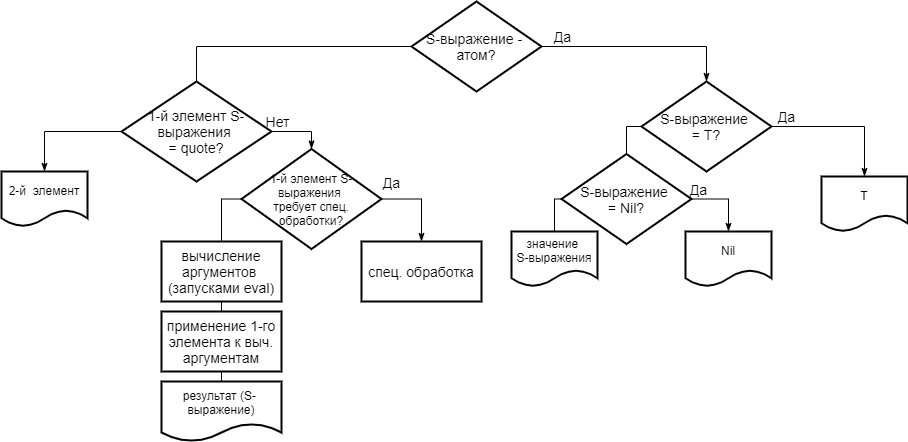
\includegraphics[scale=0.5]{img/eval}



Квотирование объекта -- это применение к нему функции quote, которая в качестве своего значения выдаёт сам аргумент, не вычисляя его. По сути, эта функция блокирует вычисление своего аргумента. Необходимость в этом нередко возникает при использовании обычных встроенных функций, чтобы задать аргументы в явном виде и избежать их вычисления. Константы–числа и атомы T, NIL при их  использовании в качестве аргументов обычных функций можно не  квотировать, поскольку значением любой константы является она сама. Функция quote используется часто, поэтому допускается упрощённый способ обращения к ней с помощью апострофа, маркирующего квотируемое выражение.


В диалекте Common Lisp для замыкания функционального аргумента встроена специальная форма (function F), где F – определяющее  выражение функции. Эту форму часто называют функциональной  блокировкой, поскольку она аналогична по действию функции quote, но  не просто квотирует аргумент, а как бы замыкает значения используемых  в функциональном аргументе F свободных переменных, фиксируя их значения из контекста его определения. Функциональную блокировку  можно записывать короче, с помощью двух знаков \#' (получить функцию с данным именем").


















\section*{Cond, if, and, or, not}

\textbf{cond}

Общий вид условного выражения:

$(cond \; (p_1  \; e_{11}  \;  e_{12}  \;  …  \;  e_{1m_1})  \;  (p_2  \;  e_{21} \;  e_{22}  \;  …  \;  e_{2m_2})  \;  …  \;  (p_n  \; e_{n1} \;  e_{n2} \;  …  \; e_{nm_n})), m_i \geqslant 0 , n \geqslant 1$

Вычисление условного выражения общего вида выполняется по  следующим правилам:

\begin{enumerate}
	\item последовательно вычисляются условия $p_1, p_2, … p_n$ ветвей выражения до тех пор, пока не встретится выражение $p_i$, значение   которого отлично от NIL;
	\item последовательно вычисляются выражения-формы $e_{i1} \;  e_{i2} \;  … \;  e_{im_i}$ соответствующей ветви, и значение последнего выражения $e_{im_i}$ возвращается в качестве значения функции cond;
	\item если все условия $p_i$ имеют значение NIL, то значением условного выражения становится NIL.
\end{enumerate}

Ветвь условного выражения может иметь вид ($p_i$), когда $m_i$ = 0. Тогда если значение pi $\neq$ NIL, значением условного выражения cond становится значение pi.

В случае, когда pi $\neq$ NIL и $m_i$ $\geqslant$ 2, то есть ветвь cond содержит более  одного выражения $e_i$, эти выражения вычисляются последовательно, и  результатом cond служит значение последнего из них $e_{im_i}$. Таким  образом, в дальнейших вычислениях может быть использовано только значение последнего выражения, и при строго функциональном  программировании случай $m_i$ $\geqslant$ 2 обычно не возникает, т.к. значения  предшествующих $e_{im_i}$ выражений пропадают. 


 
\textbf{if}

Макрофункция (If C E1 E2), встроенная в MuLisp и Common Lisp, вычисляет значение выражения E1, если значение выражения C отлично от NIL, в ином случае она вычисляет значение E2:

(defmacro If (C E1 E2) (list 'cond (list C E1) (list T E2)))

Этот макрос строит и вычисляет условное выражение cond, в котором в качестве условия первой ветви берётся выражение С (первый аргумент If), а выражения E1 и E2 (второй и третий аргумент If) размещаются соответственно на первой и второй ветви cond.


\textbf{and/or/not}

К логическим функциям-предикатам относят логическое отрицание not, конъюнкцию and и дизъюнкцию or. Первая из этих функций является обычной, а другие две – особыми, поскольку допускают произвольное количество аргументов, которые не всегда вычисляются. 

Логическое отрицание not вырабатывает соответственно: (not NIL) => T и (not T) => NIL, и может быть определено функцией (defun not (x) (eq x NIL)).


Вызов функции and, реализующей конъюнкцию, имеет вид (and e1 e2 … en), n $\geqslant$ 0. 

При вычислении этого функционального обращения последовательно слева направо вычисляются аргументы функции ei – до тех пор, пока не  встретится значение, равное NIL. В этом случае вычисление прерывается и значение функции равно NIL. Если же были вычислены все значения ei и  оказалось, что все они отличны от NIL, то результирующим значением функции and будет значение последнего выражения en .

Вызов функции-дизъюнкции имеет вид (or e1 e2 … en), n $\geqslant$ 0. 

При выполнении вызова последовательно вычисляются аргументы ei (слева направо) – до тех пор, пока не встретится значение ei, отличное от NIL. В этом случае вычисление прерывается и значение функции равно значению этого ei. Если же вычислены значения всех аргументов ei, и оказалось, что они равны NIL, то результирующее значение функции равно NIL.

При n=0 значения функций: (and)=>T, (or)=>NIL.

Таким образом, значение функции and и or не обязательно равно Т или NIL, а может быть произвольным атомом или списочным выражением.




\section*{Отличие в работе функций cons, list, append, nconс и в их результате}

cons принимает 2 указателя на любые S-выражения и возвращает новую cons-ячейку (списковую ячейку), содержащую 2 значения. Если второе значение не NIL и не другая cons-ячейка, то ячейка печатается как два значения в скобках, разделённые точкой (так называемая точечная пара). Иначе, по сути, эта функция включает значение первого аргумента в начало списка, являющегося значением второго аргумента. 

Функция list, составляющая список из значений своих аргументов (у которого голова -- это первый аргумент, хвост -- все остальные аргументы), создает столько списковых ячеек, сколько аргументов ей было передано. Эта функция относится к особым, поскольку у неё может быть произвольное число аргументов, но при этом все аргументы вычисляются.

append принимает произвольное количество аргументов-списков и соединяет (сливает)  элементы верхнего уровня всех списков в один список. Действие append иногда называют конкатенацией списков. В результате должен быть построен новый список.

Например: (append (list 1 2) (list 3 4)) ==> (1 2 3 4). 

С точки зрения функционального подхода, задача функции append - вернуть список (1 2 3 4) не изменяя ни одну из cons-ячеек в списках-аргументах (1 2) и (3 4). append на самом деле создаёт только две новые cons-ячейки, чтобы хранить значения 1 и 2, соединяя их вместе и делая ссылку из CDR второй ячейки на первый элемент последнего аргумента - списка (3 4). После этого функция возвращает cons-ячейку содержащую 1. Ни одна из входных cons-ячеек не была изменена, и результатом, как и требовалось, является список (1 2 3 4). Единственная хитрость в том, что результат, возвращаемый функцией append имеет общие cons-ячейки со списком (3 4). Таким образом, если последний переданный список будет модифицирован, то  итоговый список будет также изменен.

nconc -- это структуроразрушающая версия append. Как и append, nconc возвращает соединение своих аргументов, но строит такой результат следующим образом: для каждого непустого аргумента-списка, nconc устанавливает в cdr его последней cons-ячейки ссылку на первую cons-ячейку следующего непустого аргумента-списка. После этого она возвращает первый список, который теперь является головой результата-соединения.

Итак, отличия: cons является базисной, list, append, nconc -- нет; list, append, nconc принимают произвольное количество аргументов (причем аргументами append и nconc могут быть только списки), cons -- фиксированное (два); cons создает точечную пару или список (в зависимости от второго аргумента), list, append и nconc -- список; cons и list создают новые списковые ячейки (все), append имеет общие списковые ячейки с последним списком, nconc не создает cons-ячеек; conc является структуроразрушающей, а cons, list и append -- нет.

Пусть (setf lst1 '( a b)); (setf lst2 '(c d).



\begin{lstlisting}[language=Lisp]	
	(cons lst1 lst2) => ((A B) C D)
	lst1 => (A B)
	(list lst1 lst2) => ((A B) (C D))
	lst1 => (A B)
	(append lst1 lst2) => (A B C D)
	lst1 => (A B)
	(nconc lst1 lst2) => (A B C D)
	lst1 => (A B C D)
\end{lstlisting}



\section*{Про переменные}

Лисп работает только на указателях, поэтому все в куче

Формальные параметры -- символьные атомы. Когда задаем фактиеские параметры, должна быть выделена память. Лексическая переменная -- символьный атом. Распределение памяти автоматически в нужный момент

Можно сказать, что есть локальные и глобальные атомы (T, Nil).

Установка значения символьному атому -- setf, setq от двух аргументов value значение (другой символьный атом, самовычислимый атом, структура). value устанавливается на значение второго аргумета. Как только написали setf/setq -- организовалсяглобальный атом, то есть на все время сеанса работы. Можно менять значение по указателю, но сам атом уже выделен.

Список свойтсв -- список (динамическая структура) из (имя\_свойства значение).

let

(let ((name1 value1) ... (namen valuen)) body)

выделяется память, готовятся значения, а связывание происходит в произвольном порядке. Нельзя из value2 сослаться на value1.

В let* - последовательно, более аккуратно, можно сослаться, но она дольще.

Термин среда -- при загрузке пакета. Загрузка пакета -- загрузка интерфейса (окружение).

\section*{Еще функции}

last

(nth n lst)

(nthcdr n lst)

\textbf{remove} принимает 2 аргумента и возвращает список, заданный вторым аргументом, из которого удалены все вхождения значения первого аргумента.

\textbf{sabstitute} принимает 3 аргумента и возвращает список, заданный третьим аргументом, в котором все вхождения значения второго аргумента заменены на значение первого аргумента.


(remove el lst) -- сравнивает элементы по car-указателю очередного элемента

(member elem, lst) -- возвращает остаток списка, начиная с ячейки,  у которой кар на elem указывает.

Как повлиять на работу для поиска списка
Есть механизм ключевых слов. (совокупность ключевых параметров). Могут быть использованы значения по умолчанию

(member ‘(a b) ‘(c (a b) d) :test \#’equal) => ((a b) d)


Assoc/rassoc - для таблиц

Ассоциативная таблица (приближение к БД). -- список из точечных пар (ключ -- значение), но lisp не следит заа уникальностью ключей.

assoc (rassoc) выбирает из ассоциативного списка, заданного вторым аргументом, первую точечную пару, в которой первый (второй) элемент совпадает со значением первого аргумента. 


elem не может быть структурой, так как сравнивается по eql.

\section*{Еще инфы}

Виды списков -- одноуровневые и структурированные (элементами являются списки), смешанные и числовые.

Все стандартные функции работают только по верхнему уровню.

Ассоциативная таблица (приближение к БД). -- список из точечных пар (ключ -- значение), но lisp не следит заа уникальностью ключей.

Ассоциативная таблица (приближение к БД). -- список из точечных пар (ключ -- значение), но lisp не следит заа уникальностью ключей.


Assoc/rassoc - таблицы

Функция ASSOC выбирает из ассоциативного списка, заданного вторым аргументом, первую пару, в которой первый элемент совпадает со значением первого аргумента. Как известно, ассоциативный список представляет собой список пар. Каждый элемент ассоциативного списка - есть точеная пара (в частности - список). rassoc - по второму аргументу

(assoc 'c '((a . 1) (b . 2) (c . 3) (d . 4))) ==> (c . 3)

Множество -- неупорядоченная совокупность неповторяющихся элементов.

\#' --функциональная блокировка =function




\section*{Рекурсия}

Плохо организованная рекурсия – плохо, хорошо – хорошо и сравнима с итерацией.


Рекурсия — это ссылка на определяемый объект во время его определения. 




Надо думать:
•	Когда выйти из рекурсии
•	Как уйти в рекурсию (как меняются аргументы)
•	Как вызвать рекурсивную функцию первый раз


Классификация:

1.	Простая рекурсия (рекурсивный вызов встречается в теле функции 1 раз)
2.	Рекурсия 1 порядка (несколько раз)
3.	Взаимная рекурсия (несколько функций, вызывающие друг друга)
Стремиться к эффективному варианту

(Из лабы, в скобках -- из интернета). Существуют типы рекурсивных функций: хвостовая, дополняемая, множественная (=1 порядка Рекурсия, содержащая только одну самоссылку, называется одиночная рекурсия, в то время как рекурсия,содержащая несколько самоссылок, известна как множественная рекурсия.), взаимная рекурсия и рекурсия более высокого порядка (аргументом рекурсивного вызова является рекурсивный вызов).

Реализация рекурсии с помощью cond. 
Золотое правило – в качестве первых веток – условия выхода из рекурсии
Пример на факториале.
Если уходим в рекурсию, а собираем результаты только на выходе — это неэффективно. А если сделать предварительные действия на входе. Хвостовая рекурсия
Append всегда делает копии, поэтому в рекурсии ее использовать очень. Плохо

(defun my-member (el lst)
(cond ((nul lst) Nil)
((equal el (car lst)) t)
(t (my-member el (cdr lst)))))
(my-member ‘a ‘(b a c)) -> t
(my-member Nil ())->nil

Если переставить условия выхода, то my-member Nil ())->t

(defun my-reverse (lst)
(cond ((null. Lst) lst)
(t (append (my-reverse (cdr lst)) (cons (car lst Nil))))) 
не очень, так как собираем результат на выходе

Перепишем на хвостовую рекурсию
(defun move-to (lst result)
(cond ((null lst) result)
(t (move-to (cdr lst) (cons (car lst) result)))))

(defun. my-reverse1 (lst)
(move-to lst ())

Т.к. в Lisp используются рекурсивно определенные структуры, то рекурсия — это естественный принцип обработки таких структур. При организации рекурсии можно использовать как функции с именем, так и локально определенные с помощью лямбда выражений. Кроме этого, при организации рекурсии можно использовать функционалы или использовать рекурсивную функцию внутри функционала.



\section{Лекция}

visual prolog 5.2

продолжаем классификацию рекурсий.
Дополняемая рекурсия

\begin{lstlisting}[language=Lisp]
(defun fn (x)
	(cond 
		(end-test end_value)
		(t (_cons _add_value (fn changed_x)))))
		
; можно с ддополнительным условием
(defun fn (x)
(cond
	(end-test end_value)
	(add-test (add_fun add_val (fn changed_x)))
	(t (fn changed2_x)))
	 
; функция, которая выделяет из списка символы
(defun extracct_symbolls (lst)
	(cond 
		((null lst) Nil)
		((symbolp (car lst))
			(cons (car lst) (extract_symbols (cdr llst))))))
;car-cdr-дополлняемаяя рекурсия
(defun fn (x)
	(cond
		(end-test end_value)
		(t (commbner (fn changed_x)))
			(fn changed2_x)))
			
(defun first_member (lst)
	(cond
		((number  lst) st)
		((atom lst) Nil)
		(t (or (first_number (car lst)
			)first_number (ccdr lst)))
	)
)

; количество списковых ячеек, которые представляяют список в памяти
(defun cons_sells (lst)
	(if (atom lst) 0
		(+ (length lst)
			(reduce #'+ (mapcar #'cons_sells lst)))))
			
(defun into_one_llevel (lst rst)
	(cond ((null lst) rst)
		((atom lst) (cons lst rst))
		(t (into_one_level (cdr lst)))))
		

\end{lstlisting}

\section*{Про свойства}
(boundp'symbol) - связан ли со значением
(fboundp'symbol) - связан ли с функцией 

указатель properties - на список четной длины: имя, значение (в том числе функциональное определение)

(pufprop 'symbol property\_name propert\_value) - формировать список свойств

(remprop 'symbol property\_name) - удалить пару имя значение

(syntd-plist 'symbol) - посмотреть список свойств

\section*{Механизм ключевых слов}

Действует на все аргументы после ключевого слова до следующего ключевого  слова.

1. Необязательный параметр: \&optional

В перечислении аргументов группа аргументов предваряется \&. 

(defun tt1 (x \&optional y) (list x y))
параметр y можно не указывать, по умолчанию Nil. 

Можно указать значение по умолчанию для необязательного параметра

(defun tt2 (x \&optionall (y (+ x  1))) (list x y))

2. Произвольное количество аргументов: \&rest. Перед последним обязательным аргументов. Тоогда этот последний аргумент будет связан с хвостом

(defun average (\&rest arg)
	(/  (reduce \#'+ arg) (length arg)) 1.0)

(average 2 3 4 5) - arg со всем списком

Если бы был в начале еще ооддин аргумент, то ему было бы 2, а остальное - arg

3. \&key

(defun f1 (\&key x y) (...))

: x 1
Обычно - позиционное соответсттвие, а здесь порядок следования фактических параметров указвается именами

Это даетт указывать не все аргументы при вызове, указывать в произвольном порядке.

\section{Лекция 6}



Еще виды рекурсивных функций:

1. Хвостовая рекурсия: может быть реализована с 1 или несколькими условиями выхода.

Вообще хорошая рекурсия - когда результат не надо собирать на выходе. ХР -- когда не остается недовычисленного результата в конце.

В общем виде ХВ:


\begin{lstlisting}[language=Lisp]
(defun fun (x)
	(cond (end_test end_value)
		(t (fun changed_x))
	)
)
\end{lstlisting}

Поиск первого атома (на всех уровнях) в списке

\begin{lstlisting}[language=Lisp]
(defun first_atom (lst)
	(cond 
		((atom lst) lst)
		(t (first_atom (car lst)))
	)
)
\end{lstlisting}


Первое нечетное - не работает

\begin{lstlisting}[language=Lisp]
(defun find_first_odd (lst)
	(cond 
		((null lst) Nil)
		((odd (first_atom lst)) (first_a lst)) ; нужно ли еще проверять на то, число это или нет
		(t (find_first_odd (cdr lst)))
	)
)
\end{lstlisting}

My_nth по верхнему уровню

\begin{lstlisting}[language=Lisp]
(defun my_nth (lst n)
	(cond 
		((null lst) Nil)
		((= n 0) (car lst))
		(t (my_nth (cdr lst) (- n 1)))
	)
)
\end{lstlisting}






2. Дополняемая 

Общий вид

\begin{lstlisting}[language=Lisp]
(defun func (x)
	(cond (end_test end_value)
		(t (add_function add_value (func changed_x)))
	)
)
\end{lstlisting}


length

\begin{lstlisting}[language=Lisp]
(defun my_length (lst)
	(cond 
		((null lst) 0)
		(t (+ 1 (my_length (cdr lst))))
	)
)
\end{lstlisting}


Преобразование многоуровневогоо списка в одноуровневый

\begin{lstlisting}[language=Lisp]
(defun into_one_level (lst)
	(cond 
		((null lst) Nil)
		((atom lst) (cons lst Nil))
		(t (append 
			(int_one_level (car lst))
			(into_one_level. (cdr lst))
		))
	)
)
\end{lstlisting}



Сортировка


\begin{lstlisting}[language=Lisp]
(defun insert_help (x lst)
	(cond
		((null lst) (cons x Nil))
		((<=x (car lst)) (cons x lst))
		(t (cons (car lst) (insert_help x (cdr lst))))
	)
)

(defun sort_help (lst1 lst2)
	(cond
		((null lst1) lst2)
		(t (sort_help. (cdr lst1) (cons (car lst1) lst2)))
	)
)


(defun sort (lst) (sort_holp lst ()))
\end{lstlisting}




\begin{lstlisting}[language=Lisp]

\end{lstlisting}




\end{document}


